\begin{figure}
\centering
\begin{minipage}{.45\textwidth}

\centering
   % \resizebox{0.7\textwidth}{!}{
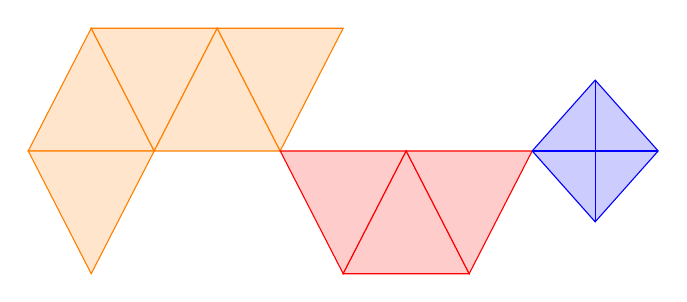
\begin{tikzpicture}[every node/.style={fill,circle,inner sep=1.5pt},yscale=0.9,xscale=0.8]

  % Define the coordinates for the shared vertices of orange triangles
  \coordinate (P1) at (0,0);
  \coordinate (P2) at (2,0);
  \coordinate (P3) at (1,1.732); % height of equilateral triangle
  \coordinate (P4) at (3,1.732);

  % Draw the orange triangles
  \filldraw[orange, fill=orange!20] (P1) -- (P2) -- (P3) -- cycle; % 1st triangle
  \filldraw[orange, fill=orange!20] (P2) -- (P3) -- (P4) -- cycle; % 2nd triangle
  \coordinate (P5) at (4,0); % Shift for the 3rd triangle
  \filldraw[orange, fill=orange!20] (P2) -- (P4) -- (P5) -- cycle; % 3rd triangle
  \coordinate (P6) at (5,1.732); % Height for the 4th triangle
  \filldraw[orange, fill=orange!20] (P4) -- (P5) -- (P6) -- cycle; % 4th triangle
  \coordinate (P7) at (1,-1.732);
  \filldraw[orange, fill=orange!20] (P1) -- (P2) --(P7) -- cycle;

  % Define the coordinates for the red triangles
  \coordinate (R1) at (5,-1.732);
  \coordinate (R2) at (6,0); 
  \coordinate (R3) at (7,-1.732);

  % Draw the red triangles
  \filldraw[red, fill=red!20] (P5) -- (R1) -- (R2) -- cycle; % 1st red triangle
  \filldraw[red, fill=red!20] (R2) -- (R1) -- (R3) -- cycle; % 2nd red triangle

  % The 3rd red triangle
  \coordinate (R4) at (8,0);
  \filldraw[red, fill=red!20] (R2) -- (R3) -- (R4) -- cycle;

  % Draw the 4-clique to the right
  \coordinate (C1) at (8,0); % Shared with 3rd red triangle
  \coordinate (C2) at (9,1);
  \coordinate (C3) at (9,-1);
  \coordinate (C4) at (10,0);
  \filldraw[blue, fill=blue!20] (R4) -- (C1) -- (C2) -- (C4) -- (C3) -- (C1); % Edges of 4-clique
  \draw[blue] (C2) -- (C3); % Diagonal of 4-clique
  \draw[blue] (C4) -- (C1); % Connect 3rd red triangle to 4-clique

  % Draw vertices of 4-clique
  % \foreach \i in {1,...,4}{
  %   \fill (C\i) circle [radius=2pt];
  % }
  % \fill (P1) circle [radius=2pt];
  % \fill (P2) circle [radius=2pt];
  % \fill (P3) circle [radius=2pt];
  % \fill (P4) circle [radius=2pt];
  % \fill (P5) circle [radius=2pt];
  % \fill (P6) circle [radius=2pt];
  % \fill (R1) circle [radius=2pt];
  % \fill (R2) circle [radius=2pt];
  % \fill (R3) circle [radius=2pt];
  % \fill (R4) circle [radius=2pt];
  % \fill (R5) circle [radius=2pt];
  
\end{tikzpicture}
         \caption{An example of hypergraph $H$. Triangles filled with colors represent hyperedges in $\hG$. Two hyperedges are 2-connected if they share two nodes. Different 2-connected components are marked in different colors. }
\label{fig:2-connectivity-H}
% \vspace{12mm}
\end{minipage}%
\hfill
\begin{minipage}{.45\textwidth}
\centering
   % \resizebox{0.7\textwidth}{!}{
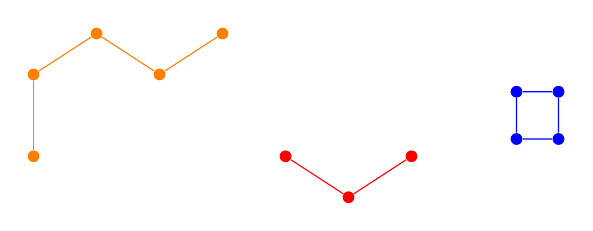
\begin{tikzpicture}[,yscale=0.9,xscale=0.8]
  % Nodes
    % Define the coordinates for the shared vertices of orange triangles
  \coordinate (P1) at (0,0);
  \coordinate (P2) at (2,0);
  \coordinate (P3) at (1,1.732); % height of equilateral triangle
  \coordinate (P4) at (3,1.732);
  \coordinate (P5) at (4,0);
  \coordinate (P6) at (5,1.732);
  \coordinate (P7) at (1,-1.732);

    % Define the coordinates for the red triangles
  \coordinate (R1) at (5,-1.732);
  \coordinate (R2) at (6,0); 
  \coordinate (R3) at (7,-1.732);

    % Draw the 4-clique to the right
  \coordinate (C1) at (8,0); % Shared with 3rd red triangle
  \coordinate (C2) at (9,1);
  \coordinate (C3) at (9,-1);
  \coordinate (C4) at (10,0);
  \coordinate (C5) at (9,0);

  \node (b1) at (barycentric cs:P1=1,P2=1,P3=1) [circle, fill=orange, inner sep=1.5pt] {};
  \node (b2) at (barycentric cs:P2=1,P3=1,P4=1) [circle, fill=orange, inner sep=1.5pt] {};
  \node (b3) at (barycentric cs:P2=1,P4=1,P5=1) [circle, fill=orange, inner sep=1.5pt] {};
  \node (b4) at (barycentric cs:P4=1,P5=1,P6=1) [circle, fill=orange, inner sep=1.5pt] {};
  \node (b5) at (barycentric cs:P1=1,P2=1,P7=1) [circle, fill=orange, inner sep=1.5pt] {};

  % Draw lines between adjacent orange barycenters
  \draw[orange] (b1) -- (b2);
  \draw[orange] (b2) -- (b3);
  \draw[orange] (b3) -- (b4);
  \draw[orange] (b1) -- (b5);

  \node (br1) at (barycentric cs:P5=1,R1=1,R2=1) [circle, fill=red, inner sep=1.5pt] {};
  \node (br2) at (barycentric cs:R2=1,R1=1,R3=1) [circle, fill=red, inner sep=1.5pt] {};
  \node (br3) at (barycentric cs:R2=1,R3=1,C1=1) [circle, fill=red, inner sep=1.5pt] {};
  \draw[red] (br1) -- (br2) -- (br3);

    \node (bc1) at (barycentric cs:C1=1,C2=1,C5=1) [circle, fill=blue, inner sep=1.5pt] {};
  \node (bc2) at (barycentric cs:C2=1,C4=1,C5=1) [circle, fill=blue, inner sep=1.5pt] {};
  \node (bc3) at (barycentric cs:C3=1,C4=1,C5=1) [circle, fill=blue, inner sep=1.5pt] {};
  \node (bc4) at (barycentric cs:C3=1,C1=1,C5=1) [circle, fill=blue, inner sep=1.5pt] {};
  \draw[blue] (bc1) -- (bc2) -- (bc3) -- (bc4) -- (bc1);
\end{tikzpicture}
         \caption{The corresponding graph $\cG_H$. Each node in $\cG_H$ corresponds to a hyperedge in $H$. Two nodes are connected if their corresponding hyperedges share two nodes.}
         % \label{fig:three sin x}
     % \end{subfigure}
% \caption{An example of  2-connectivity and 2-connected components when $d=3$.}
\label{fig:2-connectivity-G}
\end{minipage}
\end{figure}